% 
%            ,,                                        
%          `7MM            _.o9                                
%            MM                                             
%  ,6"Yb.    MM  ,p6"bo   ,6"Yb.  M"""MMV  ,6"Yb.  `7Mb,od8 
% 8)   MM    MM 6M'  OO  8)   MM  '  AMV  8)   MM    MM' "' 
%  ,pm9MM    MM 8M        ,pm9MM    AMV    ,pm9MM    MM     
% 8M   MM    MM YM.    , 8M   MM   AMV  , 8M   MM    MM     
% `Moo9^Yo..JMML.YMbmd'  `Moo9^Yo.AMMmmmM `Moo9^Yo..JMML.   
% 
% 
% Free and Open-Source template for academic works
% https://github.com/dpmj/alca



\clearpage
\cleardoublepage

\chapter{Riprogettazione in microservizi dei modelli GeneFusion}

Il principale, sebbene non l'unico, contributo sperimentale di questo lavoro di tesi magistrale è la riprogettazione in microservizi i modelli GeneFusion descritti nel Capitolo 2. Nel medesimo capitolo, al sottocapitolo 2.2, è stata proposta una potenziale ristrutturazione in due microservizi indipendenti comuni ad ambo i modelli. Lo scopo di questo capitolo è illustrare l'effettivo realizzamento di questi microservizi, e la loro messa in produzione su piattaforma Kubeflow.

\section{Containerizzazione dei microservizi dei modelli GeneFusion}

Intuitivamente, bisogna realizzare due immagini \glsname{docker} distinte, una per ogni microservizio. Le immagini Docker saranno costruite specificamente per poter accogliere le istanze sia del modello Gene Classifier, sia del modello Fusion Classifier. La realizzazione avverrà mediante Dockerfiles. Concettualmente, le immagini Docker presentano dipendenze e tecnologie diverse, che è anche il motivo della suddivisione scelta. Nella repository del progetto di tesi, è possibile osservare che la directory {\small \verb|docker-steps|} contiene due sottocartelle, una per ogni microservizio: {\small \verb|dataset|} e {\small \verb|model|}. La prima cartella contiene i file e le istruzioni per costruire l'immagine Docker relativa al microservizio Dataset Generation, mentre la seconda per il microservizio Model Training \& Testing. In ambo le cartelle potremmo quindi trovare un {\small \verb|Dockerfile|}.

\begin{code}
\captionof{listing}{Dockerfile del microservizio Dataset Generation}
\label{code:apx:a:dockerfile}
\begin{minted}{dockerfile}
# Produce un'immagine Docker parametrica che genera i dataset da dare in pasto al modello.
# Per maggiori dettagli sui singoli stage, si rimanda alla documentazione ufficiale del progetto.
    
FROM python:3.8-slim-buster as pip_dependencies
    
COPY requirements.txt ./
    
RUN pip install -r requirements.txt
    
RUN apt-get update && \
    apt-get install genometools -y --no-install-recommends
    
FROM python:3.8-slim-buster as dnabert
    
RUN apt-get update && \
    apt-get install git -y --no-install-recommends
    
RUN git clone https://github.com/jerryji1993/DNABERT && \
    cd DNABERT && \
    python3 -m pip install Cmake . && \
    python3 -m pip install --editable . && \
    cd examples && \
    cd ../.. && \
    mv DNABERT/src/transformers ./transformers && \
    rm -r DNABERT
    
FROM pip_dependencies as transcripts
    
COPY data/genes_panel.txt data/download_transcripts.py ./
    
RUN python download_transcripts.py
    
FROM ubuntu as fusim
    
RUN apt-get update && \
    apt-get install wget unzip -y --no-install-recommends
    
RUN wget https://github.com/aebruno/fusim/raw/master/releases/fusim-0.2.2-bin.zip --no-check-certificate && \
    unzip fusim-0.2.2-bin.zip && \
    rm fusim-0.2.2-bin.zip
    
RUN wget -O refFlat.txt.gz http://hgdownload.cse.ucsc.edu/goldenPath/hg19/database/refFlat.txt && \
    gunzip refFlat.txt.gz && \
    mv refFlat.txt fusim-0.2.2/refFlat.txt
    
RUN wget ftp://hgdownload.cse.ucsc.edu/goldenPath/hg19/bigZips/chromFa.tar.gz && \
    tar -xzf chromFa.tar.gz && \
    cat chr*.fa > fusim-0.2.2/hg19.fa
    
FROM pip_dependencies as core
    
COPY --from=fusim fusim-0.2.2/scripts /fusim-0.2.2/scripts
COPY --from=fusim fusim-0.2.2/fusim.jar /fusim-0.2.2/fusim.jar
COPY --from=fusim fusim-0.2.2/hg19.fa /fusim-0.2.2/hg19.fa
COPY --from=fusim fusim-0.2.2/refFlat.txt /fusim-0.2.2/refFlat.txt
    
COPY --from=dnabert transformers/ /transformers
COPY --from=transcripts transcripts/ /data/transcripts/
    
RUN apt-get update && \
    apt-get install samtools art-nextgen-simulation-tools -y --no-install-recommends && \
    samtools faidx fusim-0.2.2/hg19.fa
    
RUN apt-get install default-jre -y --no-install-recommends
    
COPY . .
    
ENTRYPOINT python gc_handler.py
\end{minted}
\end{code}

\begin{code}
\captionof{listing}{Dockerfile del microservizio Model Training \& Testing}
\label{code:apx:a:dockerfile}
\begin{minted}{dockerfile}
# Produce un'immagine Docker parametrica che effettua il training e il testing del modello.
# Per maggiori dettagli sui singoli stage, si rimanda alla documentazione ufficiale del progetto.

FROM nvidia/cuda:12.2.2-base-ubuntu22.04 as cuda

ENV DEBIAN_FRONTEND=noninteractive

RUN apt-get update && \
    apt-get install -y \
        software-properties-common && \
    add-apt-repository ppa:deadsnakes/ppa && \
    apt-get update && \
    apt-get install -y \
        git \
        curl

RUN apt-get install -y \ 
        python3.9 \
        python3.9-distutils \
        libglib2.0-0

RUN curl https://bootstrap.pypa.io/get-pip.py -o get-pip.py && \
    python3.9 get-pip.py && \
    python3.9 -m pip install --upgrade pip

RUN python3.9 -m pip install torch \
        torchvision \
        torchaudio \
        --index-url https://download.pytorch.org/whl/cu118

COPY requirements.txt ./

RUN sed -i '/torch==2.1.0+cu118/d' requirements.txt && \
    sed -i '/torchaudio==2.1.0+cu118/d' requirements.txt && \
    sed -i '/torchvision==0.16.0+cu118/d' requirements.txt

RUN python3.9 -m pip install -r requirements.txt --ignore-installed

FROM scratch as fs

COPY --from=localhost:5001/step-dataset-generation-config:latest transformers/ /transformers
COPY . .

FROM cuda as core

COPY --from=fs . .
COPY deps/transcript_label.pkl data/inputs_model/transcript_label.pkl
COPY deps/chimeric_label_fusion.pkl data/inputs_model/chimeric_label_fusion.pkl

ENTRYPOINT python3.9 gc_handler.py
\end{minted}
\end{code}

Come possiamo notare, le immagini Docker vengono costruite sfruttando una tecnica chiamata multi-stage builds (realizzata utilizzando molteplici istruzioni {\small \verb|FROM|} in un singolo {\small \verb|Dockerfile|}). Questo permette di processare step non direttamente dipendenti fra di loro in parallelo, aumentando l'efficienza del processo di costruzione. Il risultato finale, in ogni caso, non varierebbe o con senza multi-stage builds.

Le immagini Docker installano le dipendenze necessarie, sia in termini di moduli Python che in termini di software terzi o runtime, come CUDA, Fusim e GenomeTools. Un file {\small \verb|requirements.txt|} è presente per ogni microservizio, contenente esattamente le dipendenze Python necessarie per ognuno di essi. Alla fine della costruzione, l'immagine Docker viene incaricata - al momento dell'esecuzione - di eseguire il comando indicato in {\small \verb|ENTRYPOINT|}, che in questo caso corrisponde a due script Python di default che verranno, poi, sovrascritti.

E' possibile testare le immagini create con i comandi CLI {\small \verb|docker build|} e {\small \verb|docker run|}, benché questo tipo di esecuzione non assicuri effettivamente che i container vengano eseguiti organicamente e senza problemi nel contesto di Kubernetes.

\section{Bootstrap della piattaforma Kubeflow}

Come accennato, il sistema prevede un'infrastruttura \glsname{kubernetes} su cui è possibile eseguire pipeline di \glsname{ml} e deep learning, realizzata tramite \glsname{kubeflow} e sviluppata localmente con \glsname{kind}.

\begin{figure}[h]
    \centering
    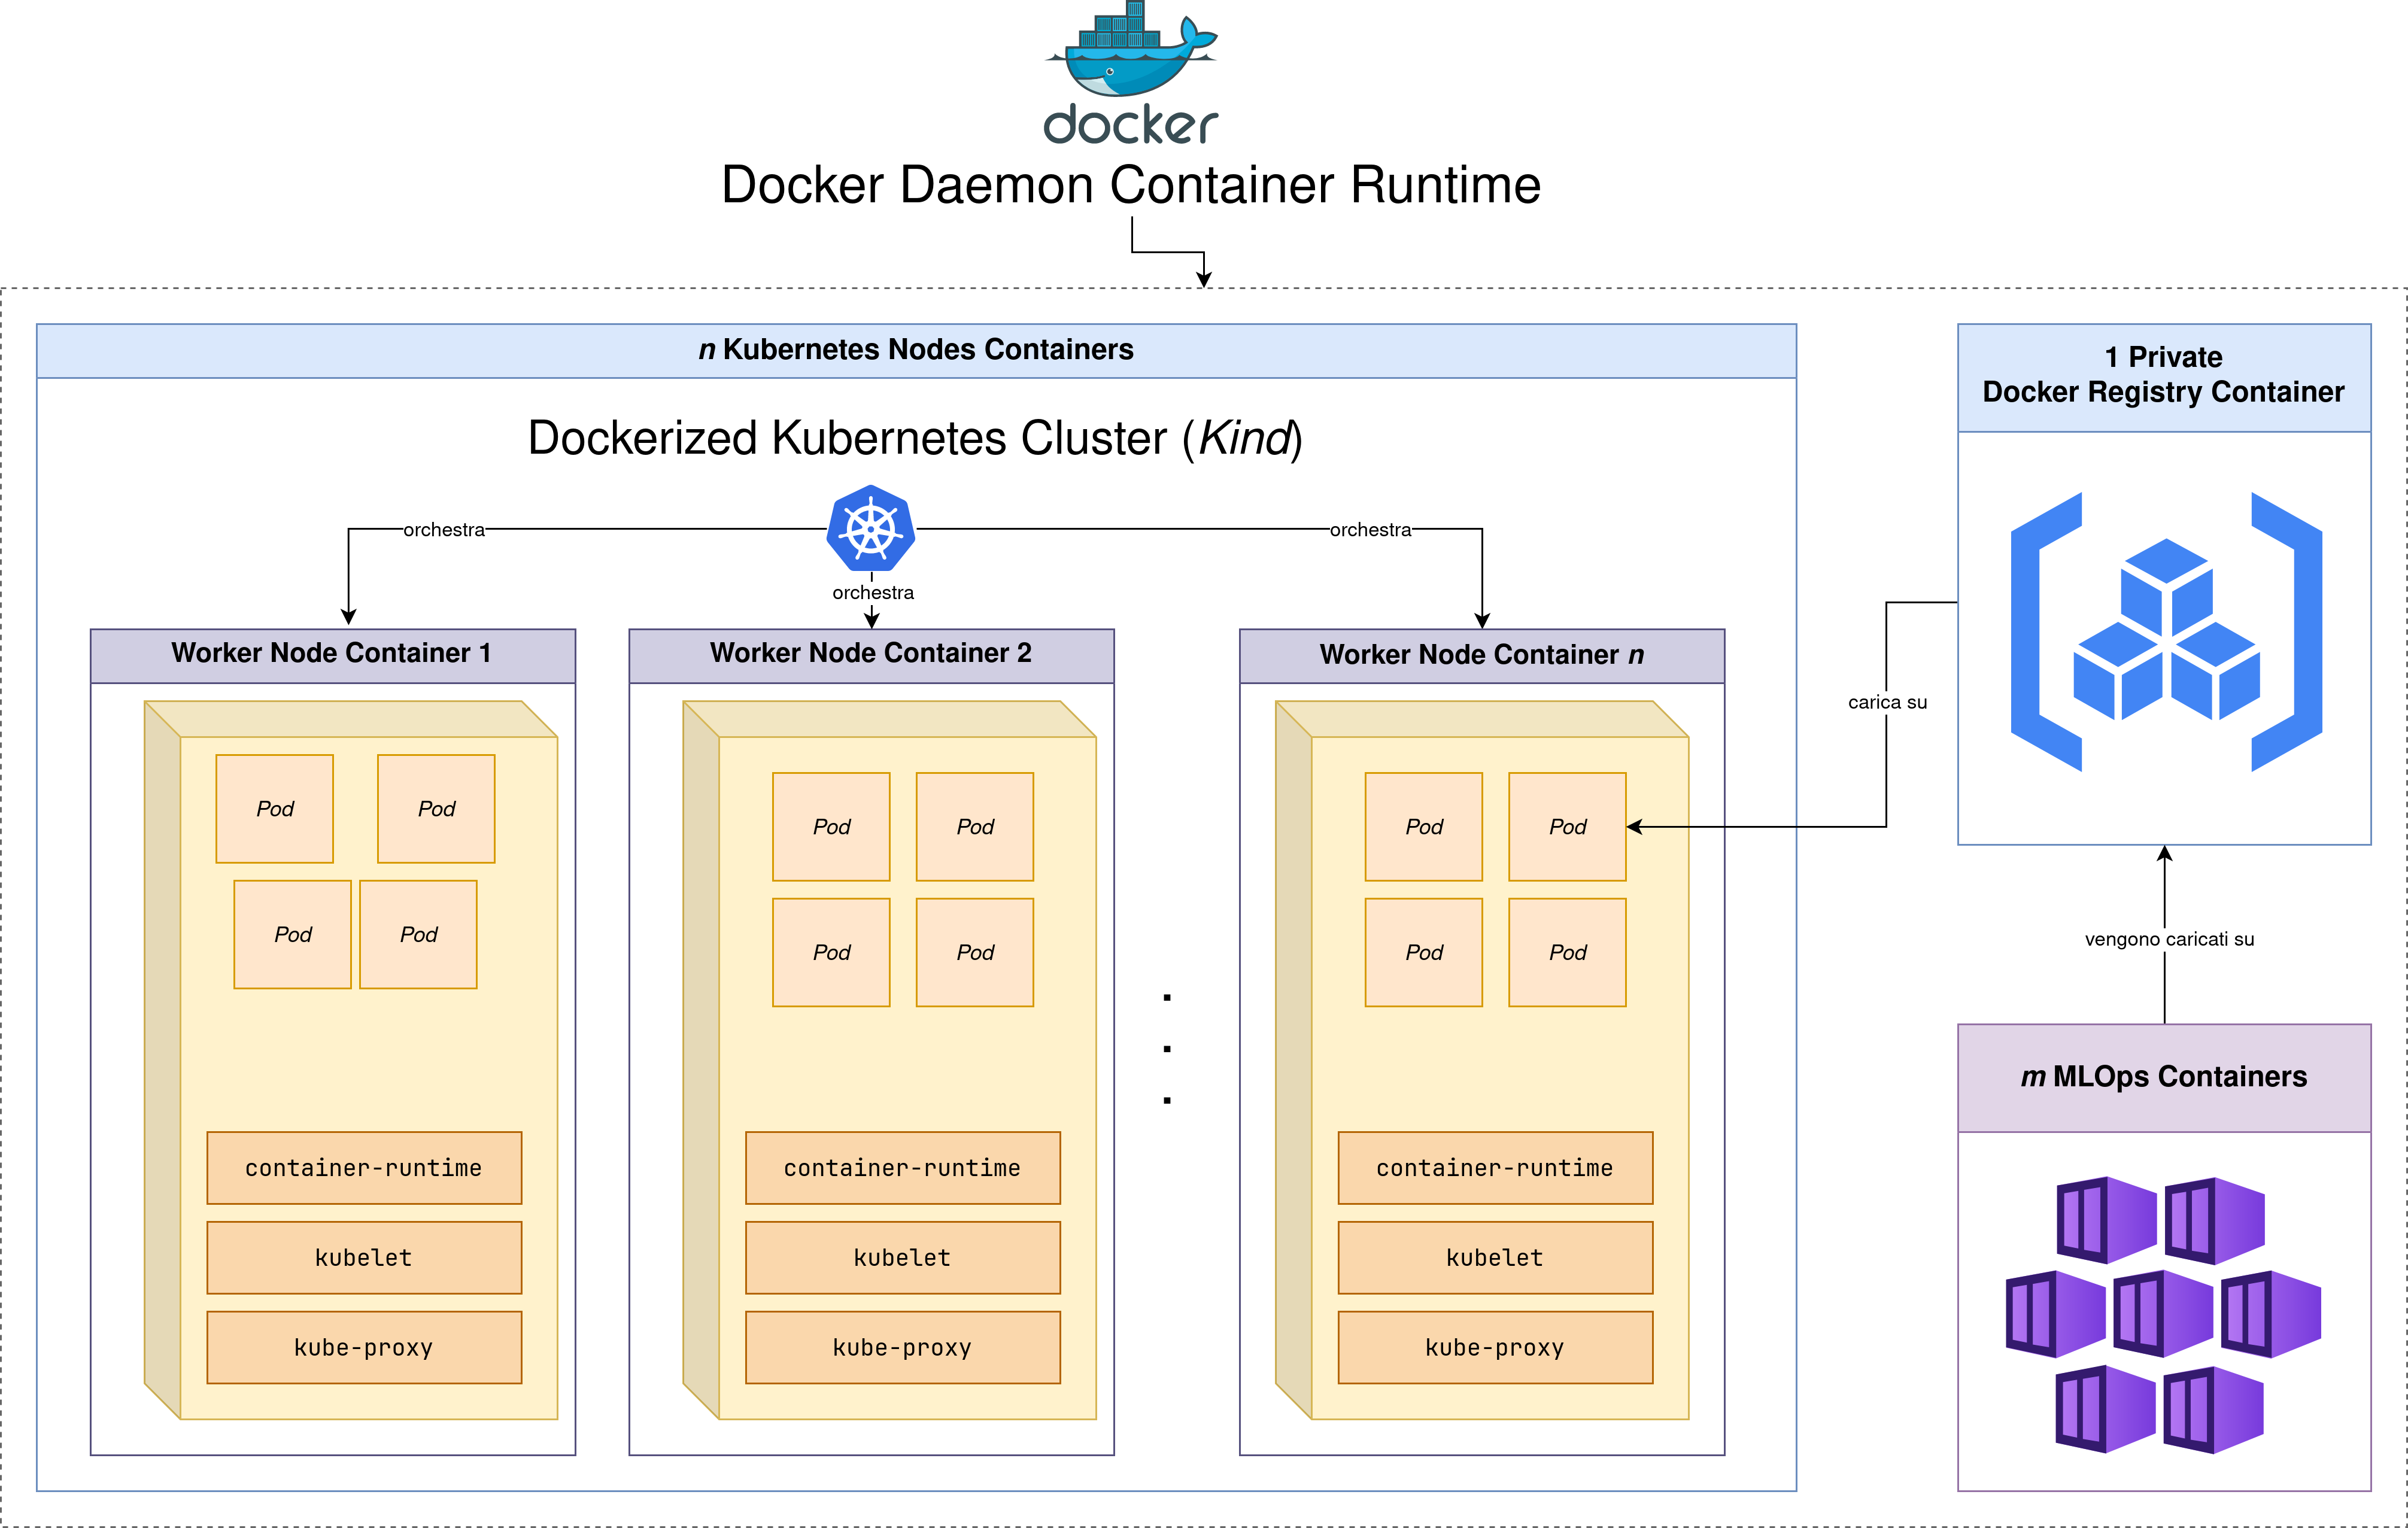
\includegraphics[width=\linewidth]{figures/ch4and5/arch.png}
    \caption[Anteprima dell'architettura realizzata]{Anteprima dell'architettura realizzata}
    \label{fig:cha6:arch}
\end{figure}

Prima di iniziare, assicurasi di aver installato sul proprio computer le seguenti dipendenze:

\begin{itemize}
    \item \glsname{docker} (v24.0.7)
    \item \glsname{kind} (v0.20.0)
    \item \glsname{helm} (v3.13.1)
    \item \glsname{kubectl} (Client v1.28.3, Server v1.27.3, Kustomize v5.0.4)
\end{itemize}

Per effettivamente creare le risorse su cui si dovrà poggiare la pipeline, e cioè le risorse legate a Kubernetes e Kubeflow, è sufficiente creare un cluster locale con Kind, e installare i manifesti Kubeflow su di esso.

\begin{small}
\begin{Verbatim}[commandchars=\\\{\}]
chmod +x kube-pipe/kind/boot-kind-gpu.sh
./kube-pipe/kind/boot-kind-gpu.sh
\textcolor{purple}{kubectl} cluster-info --context kind-kind

\textcolor{purple}{kubectl} apply -k \\ 
    "github.com/kubeflow/pipelines/manifests/kustomize/" . \\
    "cluster-scoped-resources?ref=2.0.2"
\textcolor{purple}{kubectl} wait \\
    --for condition=established \\ 
    --timeout=60s crd/applications.app.k8s.io
\textcolor{purple}{kubectl} apply -k \\ 
    "github.com/kubeflow/pipelines/manifests/kustomize/env/" . \\
    "platform-agnostic-emissary?ref=2.0.2"
\end{Verbatim}
\end{small}

Si noti che i link GitHub non dovrebbe essere troncati.

Eseguire i comandi sopraindicati avendo cura di posizionarsi prima sulla root della repository del progetto, genererà automaticamente le risorse richieste.

Sarà quindi possibile effettuare il port-forwarding della dashboard di Kubeflow col seguente comando:

\begin{small}
\begin{Verbatim}[commandchars=\\\{\}]
\textcolor{purple}{kubectl} port-forward \\ 
    -n kubeflow svc/ml-pipeline-ui \\ 
    8080:80
\end{Verbatim}
\end{small}

A questo punto, se si avrà effettuato correttamente l'installazione, su {\small \verb|localhost:8000|} sarà possibile visionare la dashboard Kubeflow.

\section{Integrazione del runtime CUDA per l'integrazione della GPU}

Il sistema, così come installato, non permetterà l'utilizzo della GPU durante le esecuzioni della pipeline, nonostante le immagini Docker realizzate già integrino coerentemente i runtime CUDA per l'utilizzo delle schede video NVIDIA.

Per integrare il runtime CUDA su Kubeflow, è necessario abilitare un operatore Kubernetes chiamato {\small \verb|gpu-operator|} che, operando tramite DeamonSets e Pods, verificherà l'effettiva presenza delle risorse hardware GPU a disponibilità dei nodi Kind.

Inoltre, è necessario istruire Docker di rendere visibile la scheda video sul proprio computer ai container in esecuzione. Per farlo, modificare il file {\small \verb|/etc/docker/daemon.json|} come segue:

\begin{code}
\captionof{listing}{Configurazione del Docker Daemon}
\label{code:apx:a:json}
\begin{minted}{json}
{
    "default-runtime": "nvidia",
    "runtimes": {
        "nvidia": {
        "args": [],
        "path": "nvidia-container-runtime"
        }
    }
}
\end{minted}
\end{code}

La modifica permetterà al Docker Daemon di rendere disponibile la GPU a tutti i container, fra cui i microservizi GeneFusion.

A questo punto, eseguire il seguente comando, che previene una serie di problemi noti legati all'incapacità di Docker di avere contezza della scheda video:

\begin{small}
\begin{Verbatim}[commandchars=\\\{\}]
\textcolor{blue}{docker} exec -ti kind-control-plane ln -s \\
    /sbin/ldconfig \\
    /sbin/ldconfig.real
\end{Verbatim}
\end{small}

Infine, utilizzando il package manager \glsname{helm}, sarà finalmente possibile installare l'operatore Kubernetes di NVIDIA, che si occuperà autonomamente di etichettare, tramite delle opportune label, le risorse allocabili sui nodi, aggiungendo la scheda video fra di essi.

\begin{small}
\begin{Verbatim}[commandchars=\\\{\}]
\textcolor{darkgreen}{helm} repo add nvidia https://helm.ngc.nvidia.com/nvidia
\textcolor{darkgreen}{helm} repo update
\textcolor{darkgreen}{helm} install --wait --generate-name \\
        -n gpu-operator --create-namespace \\
        nvidia/gpu-operator --set driver.enabled=false
\end{Verbatim}
\end{small}

E' importante confermare che le etichette siano state correttamente applicate ai nodi. Per farlo, è possibile eseguire i seguenti comandi:

\begin{small}
\begin{Verbatim}[commandchars=\\\{\}]
\textcolor{purple}{kubectl} logs \\
    -f nvidia-device-plugin-daemonset-xxx \\
    -n gpu-operator
\textcolor{purple}{kubectl} describe node kind-control-plane
\end{Verbatim}
\end{small}

\section{Caricamento delle immagini Docker su un registro on-prem}

Se la dashboard Kubeflow è effettivamente in funzione, è possibile procedere adesso al caricamento delle immagini Docker dei microservizi all'interno del registro Docker on-prem dell'architettura (realizzato mediante i comandi soprastanti). Intuitivamente, questo viene fatto poiché la pipeline Kubeflow (che risiede in uno o più container Docker nella forma di pod Kubernetes) non ha contezza delle immagini Docker presenti sull'host.

In ogni caso, eseguire i seguenti comandi costruirà le immagini Docker mediante la {\small \verb|docker build|} API, per poi pubblicarle interamente (come TAR o blobfiles) sul registro Docker di Kubeflow, mediante la {\small \verb|docker push|} API.

\begin{small}
\begin{Verbatim}[commandchars=\\\{\}]
\textcolor{blue}{docker} build \\
    -t localhost:5001/step-dataset-generation-config:latest \\
    ./docker-steps/dataset && \\
\textcolor{blue}{docker} push \\
    localhost:5001/step-dataset-generation-config:latest
\end{Verbatim}
\end{small}

\begin{small}
\begin{Verbatim}[commandchars=\\\{\}]
\textcolor{blue}{docker} build \\
    -t localhost:5001/step-model-config:latest \\
    ./docker-steps/dataset && \\
\textcolor{blue}{docker} push \\
    localhost:5001/step-model-config:latest
\end{Verbatim}
\end{small}

Il terminale dovrebbe notificare lo sviluppatore del completamento del processo, dopo il quale i microservizi saranno effettivamente visibili a Kubeflow, e integrabili in una pipeline.

\section{Creazione e compilazione della pipeline Kubeflow}

Concettualmente, l'obiettivo è realizzare due pipeline distinte (una per ogni modello), le quali applicheranno i microservizi realizzati per generare una macchina a stati che è esattamente quella proposta al Capitolo 2.2. Per raggiungere questo obiettivo, bisogna innanzitutto definire i componenti Kubeflow dei due microservizi. In questo contesto, il rateo fra componenti e microservizi non è 1:1. Facendo riferimento alla Figura 2.5, ogni "stato" (i.e. ogni rettangolo del diagramma) corrisponde ad un componente. Ciò significa che per il modello Gene Classifier si creeranno 5 componenti, mentre per il modello Fusion Classifier se ne creeranno 8, tre dei quali riusabili dal primo modello. In generale, i componenti Kubeflow, come descritto nel Capitolo 3, sono file YAML che descrivono l'implementazione dello step (come l'immagine Docker da usare) e l'interfaccia I/O. Per il resto, Kubeflow si occuperà autonomamente di trasferire gli artefatti da uno step all'altro.

Ad esempio, i due snippet che seguono mostrano due tipici componenti della pipeline. Ulteriori esempi sono rinvenibili nella repository alla directory {\small \verb|/kube-pipe/components|}.

\begin{code}
\captionof{listing}{Fusion Classifier Test Dataset Generation Component}
\label{code:apx:a:yaml}
\begin{minted}{yaml}
name: Fusion Classifier Test Dataset Generation
description: Genera il dataset di testing del modello FC

outputs:
- {name: csv_path, type: String, description: 'Test CSV path.'}

implementation:
    container:
    image: localhost:5001/step-dataset-generation-config:latest
    command: [
        python,
        'fc_handler.py',
        -type,
        test,
        -csv_path, 
        {outputPath: csv_path}
    ]
\end{minted}
\end{code}

\begin{code}
\captionof{listing}{Fusion Classifier Model Training Generation Component}
\label{code:apx:a:yaml}
\begin{minted}{yaml}
name: Fusion Classifier Model Training
description: Effettua l'addestramento del modello FC

inputs:
- {name: train_csv_path, type: String, description: 'Training CSV path.'}
- {name: val_csv_path, type: String, description: 'Validation CSV path.'}
- {name: gc_model_path, type: String, description: 'Absolute path of the Gene Classifier H5 model.'}

outputs:
- {name: model_path, type: String, description: 'H5 Model path.'}

implementation:
    container:
    image: localhost:5001/step-model-config:latest
    command: [
        python3.9,
        'fc_handler.py',
        -gc_model_path, 
        {inputPath: gc_model_path},
        -train_csv_path, 
        {inputPath: train_csv_path},
        -val_csv_path, 
        {inputPath: val_csv_path},
        -model_path, 
        {outputPath: model_path}
    ]
\end{minted}
\end{code}

A partire da questi componenti Kubeflow, è adesso possibile compilare le due pipeline eseguendo rispettivamente:

\begin{itemize}
    \item {\small \verb|compile_gene_classifier_pipeline.py|} 
    \item {\small \verb|compile_fusion_classifier_pipeline.py|}
\end{itemize}

Il prodotto della compilazione è a sua volta un file YAML.

Per eseguire i due script di compilazione, ci sono due possibilità: utilizzare \glsname{docker}, o utilizzare \glsname{miniconda}. 

\subsection{Compilazione mediante Docker}

L'utilizzo di Docker a questo punto è immediato. E' sufficiente costruire un'immagine che contenga le dipendenze Python necessarie utilizzando le istruzioni fornite in uno specifico Dockerfile.

\begin{small}
\begin{Verbatim}[commandchars=\\\{\}]
\textcolor{blue}{docker} build \\
    -t flow \\
    -f kube-pipe/flow.Dockerfile kube-pipe && \\
\textcolor{blue}{docker} run \\
    -v ./kube-pipe/relics:/relics flow \\
    compile_gene_classifier_pipeline.py
\end{Verbatim}
\end{small}

\begin{code}
\captionof{listing}{Immagine Docker per compilare le pipeline Kubeflow}
\label{code:apx:a:dockerfile}
\begin{minted}{dockerfile}
# Produce un'immagine Docker per la compilazione delle pipeline Kubeflow.

FROM python:3.8-slim-buster

COPY requirements.txt ./

RUN pip install -r requirements.txt

COPY . .

ENTRYPOINT ["python"]
\end{minted}
\end{code}

\subsection{Compilazione mediante Miniconda}

In alternativa, è possibile generare un ambiente virtuale Python on-the-fly usando \glsname{miniconda}. E' sufficiente creare un ambiente Conda con Python 3.8.18, attivarlo e installare i moduli richiesti. Alla fine dell'installazione delle dipendenze, sarà sufficiente eseguire gli script Python sopraindicati.

\begin{small}
\begin{Verbatim}[commandchars=\\\{\}]
conda create -n kf python=3.8.18
conda activate kf
pip install -r kube-pipe/requirements.txt
python kube-pipe/compile_gene_classifier_pipeline.py
\end{Verbatim}
\end{small}

\subsection{Caricamento della pipeline su Kubeflow}

Al di là di come si sceglie di generare i file YAML a seguito della compilazione delle pipeline, sarà possibile caricare direttamente il file (che descrive la macchina a stati della pipeline) tramite la UI della dashboard di Kuberflow.

\begin{figure}[H]
    \centering
    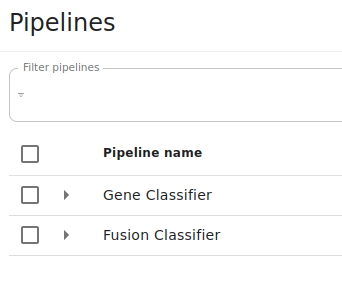
\includegraphics[width=200px]{figures/ch4and5/pp.png}
    \caption[Pipeline sulla dashboard di Kubeflow]{Pipeline sulla dashboard di Kubeflow}
    \label{fig:cha6:pp-ui}
\end{figure}

Ad un primo caricamento, si ottiene un overview del risultato finale.

\begin{figure}[H]
    \centering
    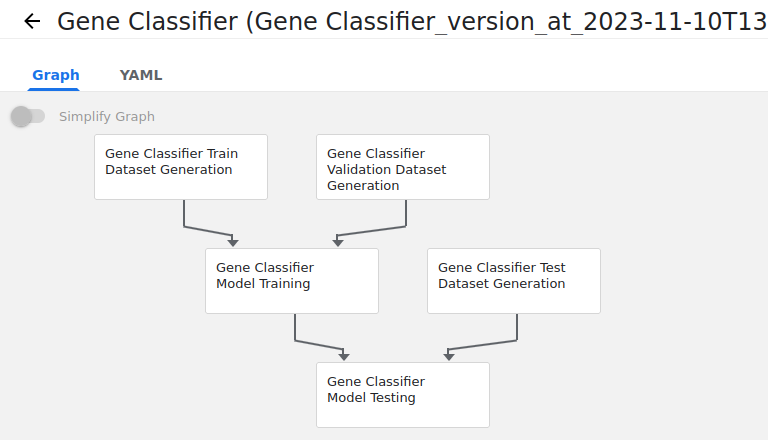
\includegraphics[width=\linewidth]{figures/ch4and5/stale.png}
    \caption[Prospetto della macchina a stati del modello Gene Classifier]{Prospetto della macchina a stati del modello Gene Classifier}
    \label{fig:cha6:stale}
\end{figure}

\begin{figure}[h]
    \centering
    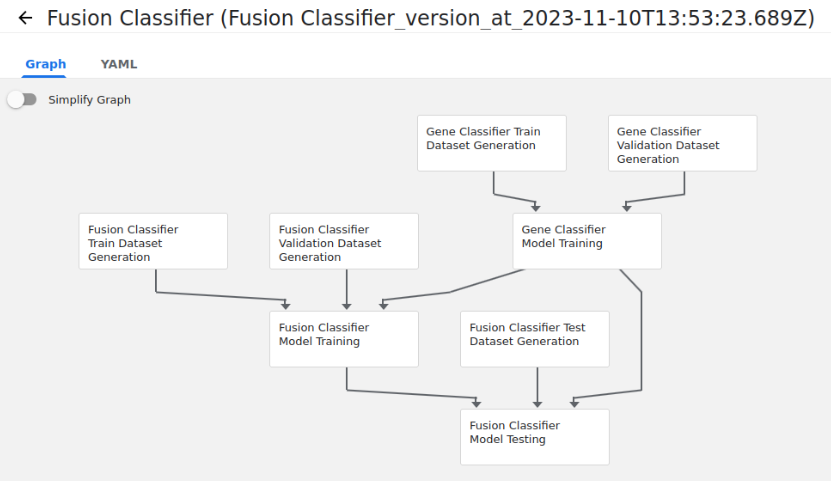
\includegraphics[width=\linewidth]{figures/ch4and5/fusion_stale.png}
    \caption[Prospetto della macchina a stati del modello Fusion Classifier]{Prospetto della macchina a stati del modello Fusion Classifier}
    \label{fig:cha6:fusion_stale}
\end{figure}

E' anche possibile effettuare versioning delle pipeline, attraverso nuovi caricamenti del manifesto YAML.

\begin{figure}[h]
    \centering
    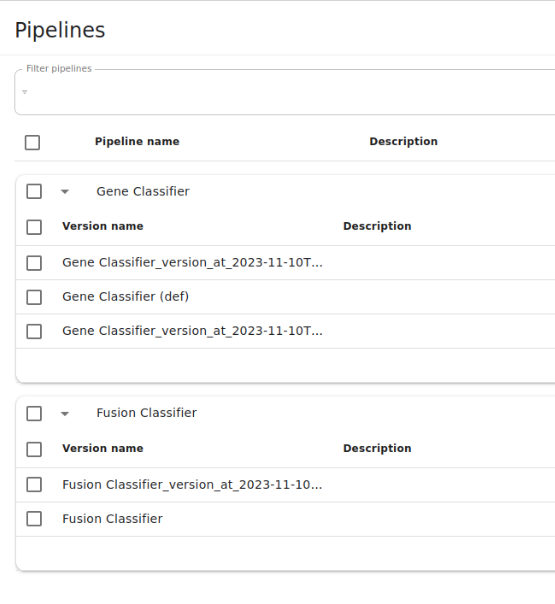
\includegraphics[width=350px]{figures/ch4and5/vers.png}
    \caption[Versioning delle pipelines]{Versioning delle pipelines}
    \label{fig:cha6:versions}
\end{figure}

\section{Esecuzione della pipeline}

Interagendo con la UI della dashboard di Kuberflow, sarà possibile avviare delle esecuzioni delle macchine a stati appena caricate. 

Dal menù principale, è possibile visionare tutte le esecuzioni avviate, e il loro risultato.

\begin{figure}[H]
    \centering
    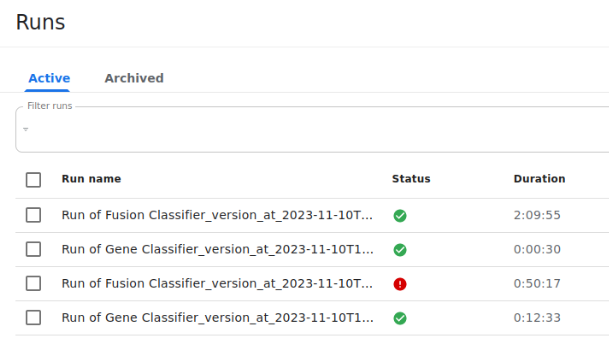
\includegraphics[width=350px]{figures/ch4and5/runs.png}
    \caption[Lista delle esecuzioni delle pipeline]{Lista delle esecuzioni delle pipeline}
    \label{fig:cha6:runs}
\end{figure}

Gli artefatti in output saranno salvati in una schermata indipendente, benché visibili anche durante le esecuzioni.

\begin{figure}[H]
    \centering
    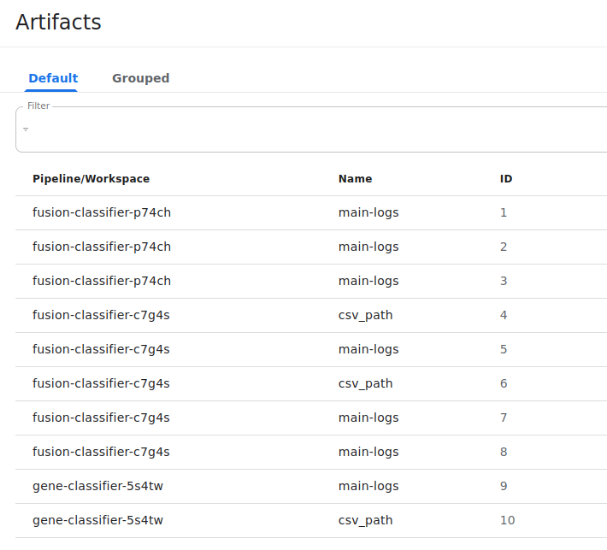
\includegraphics[width=350px]{figures/ch4and5/artifacts.png}
    \caption[Artefatti delle esecuzioni delle pipeline]{Artefatti delle esecuzioni delle pipeline}
    \label{fig:cha6:art}
\end{figure}

L'avvio di una nuova esecuzione genererà nuovi pod (con una speciale configurazione chiamata Job) all'interno del cluster Kind. Questi nuovi pod sono analizzabili come qualsiasi altra risorsa Kubernetes. E' altresì banale osservare come ogni step della macchina a stati corrisponda, di per sé, ad un nuovo pod.

Se i componenti e la pipeline sono stati configurati correttamente, allora l'esecuzione procederà organicamente, rilasciando artefatti intermedi alla fine di ogni step, e mappando l'output e gli input degli step così come descritto nei manifesti YAML.

\begin{figure}[H]
    \centering
    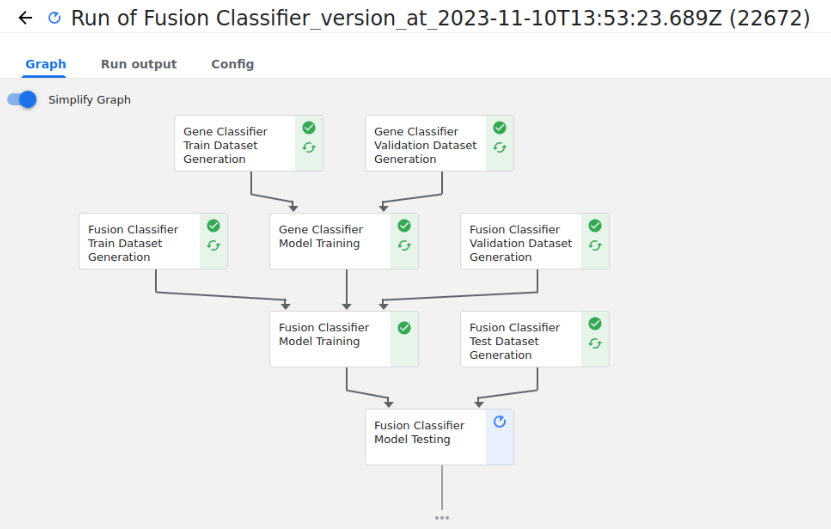
\includegraphics[width=\linewidth]{figures/ch4and5/fusion_pending.png}
    \caption[Esecuzione in corso della pipeline del modello Fusion Classifier]{Esecuzione in corso della pipeline del modello Fusion Classifier}
    \label{fig:cha6:kf-f-pend}
\end{figure}

L'STDOUT e l'STDERR per ogni container dei pod sono consultabili direttamente dalla UI. Da qui, è possibile tener traccia dell'andamento dell'esecuzione.

L'andamento della pipeline è facilmente intuibile dagli indicatori blu, rossi e verdi posizionati agli angoli di ogni step.

\begin{figure}[H]
    \centering
    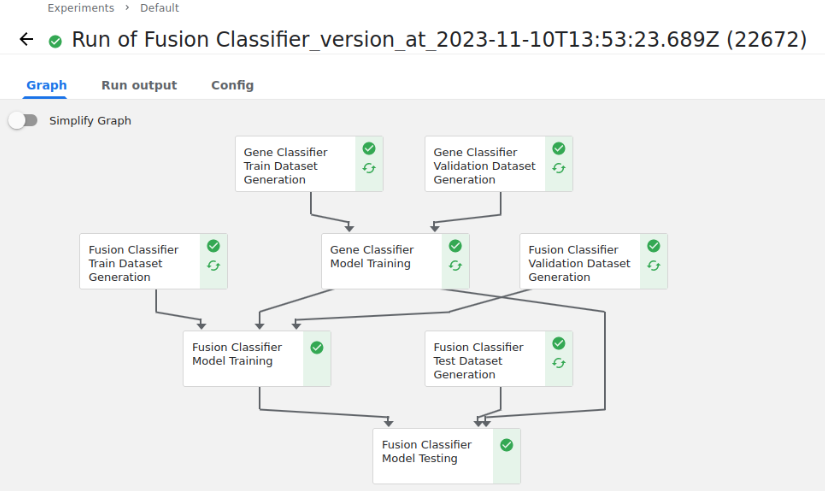
\includegraphics[width=\linewidth]{figures/ch4and5/fusion_compl.png}
    \caption[Esecuzione completata della pipeline del modello Fusion Classifier]{Esecuzione completata della pipeline del modello Fusion Classifier}
    \label{fig:cha6:kf-f-done}
\end{figure}

Alla fine dell'esecuzione, l'output finale (file CSV nel caso dei modelli GeneClassifier) sono visualizzabili come un generico artefatto scarabile.

\begin{figure}[H]
    \centering
    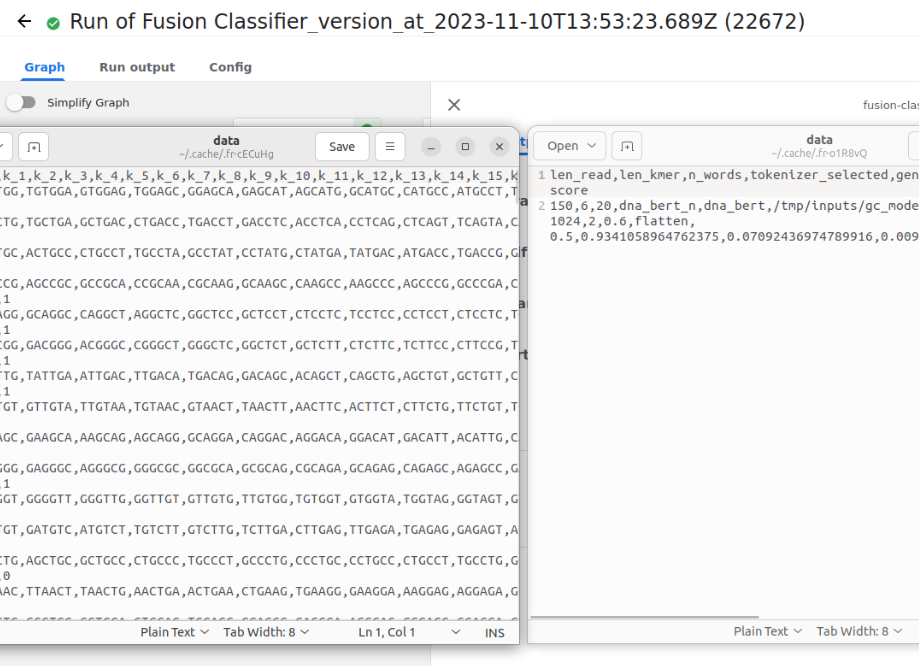
\includegraphics[width=350px]{figures/ch4and5/output.png}
    \caption[Output delle esecuzioni delle pipeline]{Output delle esecuzioni delle pipeline}
    \label{fig:cha6:kf-output}
\end{figure}

\section{Benchmark delle prestazioni}

Per effettivamente tarare l'efficienza e le performance della nuova architettura a microservizi realizzata, rispetto alla precedente architettura monolitica dei modelli GeneFusion, è stata realizzata un'immagine Docker di quest'ultima, da confrontare con una esecuzione vergine su Kubeflow della pipeline.

\begin{code}
\captionof{listing}{Dockerfile del monolite dei modelli GeneFusion}
\label{code:apx:a:dockerfile}
\begin{minted}{dockerfile}
# Produce un'immagine Docker dei modelli monolitici originali GeneFusion.

# Fusim Tools
FROM ubuntu as fusim

RUN apt-get update && \
    apt-get install wget unzip -y --no-install-recommends

RUN wget https://github.com/aebruno/fusim/raw/master/releases/fusim-0.2.2-bin.zip --no-check-certificate && \
    unzip fusim-0.2.2-bin.zip && \
    rm fusim-0.2.2-bin.zip

RUN wget -O refFlat.txt.gz http://hgdownload.cse.ucsc.edu/goldenPath/hg19/database/refFlat.txt && \
    gunzip refFlat.txt.gz && \
    mv refFlat.txt fusim-0.2.2/refFlat.txt

RUN wget ftp://hgdownload.cse.ucsc.edu/goldenPath/hg19/bigZips/chromFa.tar.gz && \
    tar -xzf chromFa.tar.gz && \
    cat chr*.fa > fusim-0.2.2/hg19.fa

# DNA-BERT Transformer
FROM python:3.8-slim-buster as dnabert

RUN apt-get update && \
    apt-get install git -y --no-install-recommends

RUN git clone https://github.com/jerryji1993/DNABERT && \
    cd DNABERT && \
    python3 -m pip install Cmake . && \
    python3 -m pip install --editable . && \
    cd examples && \
    cd ../.. && \
    mv DNABERT/src/transformers ./transformers && \
    rm -r DNABERT

# Main Stage - CUDA
FROM nvidia/cuda:12.2.2-base-ubuntu22.04 as cuda

ENV DEBIAN_FRONTEND=noninteractive

RUN apt-get update && \
    apt-get install -y \
        software-properties-common && \
    add-apt-repository ppa:deadsnakes/ppa && \
    apt-get update && \
    apt-get install -y \
        git \
        curl

RUN apt-get install -y \ 
        python3.9 \
        python3.9-distutils \
        libglib2.0-0

RUN curl https://bootstrap.pypa.io/get-pip.py -o get-pip.py && \
    python3.9 get-pip.py && \
    python3.9 -m pip install --upgrade pip

RUN apt-get update && \
    apt-get install genometools samtools art-nextgen-simulation-tools -y --no-install-recommends

RUN apt-get install default-jre -y --no-install-recommends

RUN python3.9 -m pip install torch \
        torchvision \
        torchaudio \
        --index-url https://download.pytorch.org/whl/cu118

RUN git clone https://github.com/antoniogrv/kubeless-gf.git

WORKDIR /kubeless-gf

RUN sed -i '/torch==2.1.0+cu118/d' requirements.txt && \
    sed -i '/torchaudio==2.1.0+cu118/d' requirements.txt && \
    sed -i '/torchvision==0.16.0+cu118/d' requirements.txt

RUN python3.9 -m pip install -r requirements.txt --ignore-installed

RUN python3.9 data/download_transcripts.py

COPY --from=fusim fusim-0.2.2/scripts fusim-0.2.2/scripts
COPY --from=fusim fusim-0.2.2/refFlat.txt fusim-0.2.2/refFlat.txt
COPY --from=fusim fusim-0.2.2/fusim.jar fusim-0.2.2/fusim.jar
COPY --from=fusim fusim-0.2.2/hg19.fa fusim-0.2.2/hg19.fa

COPY --from=dnabert transformers/ transformers

RUN samtools faidx fusim-0.2.2/hg19.fa

ENTRYPOINT ["python3.9", "train_gene_classifier.py"]
\end{minted}
\end{code}

Il test è stato tarato su esecuzioni dummy per il modello Gene Classifier.

\begin{table}[h]
\centering
\caption*{Benchmark delle prestazioni}
\begin{tabular}{|l|l|}
\hline
\textbf{Architettura} & \textbf{Tempo di esecuzione per il modello GC} \\ \hline
Microservizi & 12m33s \\ \hline
Monolite & 15m19s \\ \hline
\end{tabular}
\end{table}

Si è rilevato un miglioramento del 22.05\%, dovuto prevalentemente alla parallelizzazione degli step di generazione dei dataset.